\documentclass[UTF8]{ctexart}
\usepackage{geometry} %页面设置
\usepackage{indentfirst} %段落缩进设置
\usepackage{chngpage} %可以设置段落整体左右缩进等等,方法是\begin{adjustwidth}{1em}{0em}
\usepackage{iitem} %多重列表
%\usepackage{mathabx} %数学符号,与amsmath冲突
\usepackage{amsmath} %公式中输入汉字,与amssymb配合可以输入比\ge更美观的大于等于号
\usepackage{float}
\usepackage{amssymb,amsfonts}
\usepackage{mathrsfs}
%section和subsection新起一页
\usepackage{caption} %取消figure下的编号
\usepackage{titlesec}
\newcommand{\sectionbreak}{\clearpage}
%\newcommand{\subsectionbreak}{\clearpage}

%定义一个强调格式,红色加粗,使用方法\qd{你的内容},或者\begin{qds} 你的内容 \end{qds}
\usepackage{color}
\newcommand \qds {\bf \color{red}}
\newcommand \qd[1] {\begin{qds} {#1} \end{qds}}

%设置文档页面布局、字体、段落首行缩进、段间距
\setCJKmainfont{微软雅黑}
\geometry{a4paper,left=1cm,right=1cm,top=2cm,bottom=2cm}
 \setlength{\parindent}{0em}
 \setlength{\parskip}{1em}
 \usepackage{listings} %插入代码  
\usepackage{xcolor} %代码高亮  
   
\lstset{numbers=left, %设置行号位置  
        numberstyle=\tiny, %设置行号大小  
        keywordstyle=\color{blue}, %设置关键字颜色  
        commentstyle=\color[cmyk]{1,0,1,0}, %设置注释颜色  
        frame=single, %设置边框格式  
        escapeinside=``, %逃逸字符(1左面的键),用于显示中文  
        breaklines, %自动折行  
        extendedchars=false, %解决代码跨页时,章节标题,页眉等汉字不显示的问题  
        xleftmargin=2em,xrightmargin=2em, aboveskip=1em, %设置边距  
        tabsize=4, %设置tab空格数  
        showspaces=false %不显示空格  
       }  

\title{《固定收益建模》读书笔记}
\author{john107}
\date{\today}
\begin{document}

\maketitle
\clearpage
\tableofcontents
\clearpage
\section{概述}
许多固定收益证券的价格都通过各种利率和收益率来表示,所以了解固定收益定价等同于了解利率的行为。利率期限结构是固定收益分析和利率变动中的关键概念

利率期限结构被定义为利率与不同到期期限之间的依存关系

无套利机会是金融资产定价的基石,因为一个存在套利机会的市场不是一个处于均衡状态的市场

对于给定的年利率,计算利息的频率越高,得到的“有效”利率也就越高

\subsection{债券类型}
零息债券(zero-coupon bonds)和附息债券(coupon bonds)

息票率也被称为票面利率或标称利率

大多数债券都是所谓的子弹债券(bullet bonds)或纯粹附息债券(straight-coupon bonds),也就是说,在最后支付之前的所有单次支付等于债券面值与息票率的乘积

有一种债券叫年金债券(annuity bonds),每个支付日支付的金额都是相等的,每次偿还的本金逐渐增加

\begin{itemize}
\item{还款额计算关键:最后一期的本息之和等于固定还款额}
\end{itemize}

有些债券是所谓的分期还本债券(serial bonds),这种债券的本金以等额分期偿还。

\begin{itemize}
\item{还款额计算关键:每期还的本金为1/n,剩余略}
\end{itemize}

最后,少数债券是永久债券(perpetuities或consols)。这种债券只偿付利息,不偿付本金,没有到期日

大多数附息债券的票面利率是固定的,但是也有少数债券的票面利率在债券的存续期内进行定期的重设。这种债券成为浮动利率债券(floating rate bonds)

在大多数市场中,只有少数的零息债券在交易

\subsection{债券收益率和零息票利率(即期利率)}
即期利率(spot rate)是从设定时刻开始的一段时间内适用的利率

债券的收益率(yield)是使得债券全部未来支付的现值等于当前债券价格的贴现率

到期日为T的零息债券收益率(zero-coupon yield),也叫零息债券利率(zero-coupon rate)或即期利率

作为到期日的函数的零息债券利率被称为零息债券收益率曲线(zero-coupon curve),或简单地称为收益率曲线(yield curve)。收益率曲线是一种表示利率期限结构的方法。

由于在零息债券价格和零息债券收益率之间存在一一对应的关系,贴现函数$T \mapsto B^T_t$和零息债券收益率曲线$T \mapsto \hat y_t^T$之间包含了完全相同的信息。

对于年利率R,如果一年m次复利,与其对应的年贴现因子则是$(1+R/m)^{-m}$。反过来,与之相对应的一年m次复利的实际利率是$(1+R/m)^m-1$。与通常的名义利率相对应,这一利率有时被称为“有效利率”。这是国际货币市场设定贷款利率的典型惯例。国际货币市场最常使用的利率是伦敦银行同业拆借利率(London interbank offered rate, LIBOR)。对市场上LIBOR利率驳价,应当按照上述方式使用。

随着复利频率m的增加,以R的年利率投资1美元,1年的有效回报增加至$e^R$,因$\lim\limits_{m\rightarrow \infty}(1+R/m)^m=e^R$。一个连续复利的名义利率R等价于年复利$e^R-1$(这一利率大于R)。相似地,零息债券的价格$B_t^T$与连续复利的债券收益率之间满足关系式$$B_t^T=e^{-y^T_t(T-t)}$$
(可以按分数形式来理解,折现率=PV/FV),也就是$$y_t^T=-\frac {1} {T-t}ln B_t^T$$

函数$T \mapsto y_t^T$同样是零息债券收益率曲线,它包含了与贴现函数$T \mapsto B_t^T$以及年复利收益率曲线$T \mapsto \hat y_t^T$(或者说具有任何其他不同复利频率的收益率曲线)相同的信息。在连续复利和年复利零息债券收益率之间存在以下关系:$$y_t^T=ln(1+\hat y_t^T)$$考虑到数学处理上的便利性,我们在大多数模型中将重点讨论连续复利收益率问题。

\subsection{远期利率}

零息债券的收益率或即期利率反映的是从现在开始到未来某一天到期的一笔贷款的价格,远期利率所反映的则是两个未来日期之间的贷款价格。我们用$\hat f_t^{T,S}$来表示t时刻时间T与时间S之间的复利远期利率。在次,我们规定$t \leq T < S$。这个远期利率就是t时刻,我们在时间T和S之间所能采用的合适的贴现率。如果我们要从时间S贴现到t,可以先从S贴现到T,再从T贴现到t。因此,我们必定有:$$(1+\hat y_t^S)^{-(S-t)} = (1+\hat y_t^T)^{-(T-t)} (1+\hat y_t^{T,S})^{-(S-T)} $$从中我们可以得出$$\hat f_t^{T,S}=\frac {(1+\hat y_t^T)^{-(T-t)/(S-T)}} {(1+\hat y_t^S)^{-(S-t)/(S-T)}} -1 $$
同样,我们可以将上式用零息债券价格的形势表示为$$B_t^S=B_t^T(1+^hat f_t^{T,S})^{-(S-T)}$$因此,远期利率由下式给出:$$\hat f_t^{T,S}=(\frac{B_t^T}{B_t^S})^{1/(S-T)}-1$$
我们把从T时刻起的无限短的区间里的远期利率简单称为T时刻的远期利率,并将其定义为$f_t^T=\lim_{S \rightarrow T}f_t^{T,S}$。函数$T \mapsto f_t^T$被称为远期利率期限结构(term structure of forward rates)或远期利率曲线(forward rate curve)

远期利率反映了零息债券收益率曲线的斜率。特别是,当且仅当零息债券收益率曲线在T有水平切线时,远期利率$f_t^T$与零息债券收益率$y_t^T$相等。因为$$f_t^T=y_t^T+\frac{\partial y_t^T}{\partial T}(T-t)$$证明自己思考,不难,注意参考零息债券价格。

\subsection{利率期限结构的其他面具}
贴现因子、即期利率和远期利率(以任何频率计算复利)在表达相同的信息方面是完全等价的。学术界经常使用连续复利,因为使用数学指数表示相关计算可以更简洁。但连续复利收益率可以很容易地转化为任何其他复利频率。

由于大多数债券都是子弹型债券,许多人都习惯于用子弹型债券收益率的方式,而不是贴现因子或零息债券收益率的方式去思考问题。对于一个给定的到期日,平价收益率(par yield)就是使得该子弹型债券的价格等于其面值的票面利率。我们需要将付息周期固定下来,通常假设半年付息一次,类似美国国债。

评价收益率与所谓的互换利率(swap rate)之间具有比较紧密的联系。互换利率是互换市场的一个重要概念。

\subsection{债券市场和货币市场}
美国国债分成短期国债(T-bills)、中期国库票据(T-notes)和长期国库债券(T-bonds)3类,其中短期国债到期日为1年以内,中期国库票据一般在1-10年到期,长期国库债券到期为10年和30年两种。

地方政府也可以发行债券,在美国,这样的债券就是市政债券。

美国的公司债的期限通常是10-30年,而且通常是可赎回债券(callable bond)。

大部分按揭有一个提前还款的期权,就是说在贷款期间,借款人有权提前偿还所有未偿付本息。

发行人或其他机构都可以将按揭贷款汇集在一起,然后发行对该按揭贷款池具有所有权的按揭抵押债券。最常见的按揭抵押债券的形式就是过手证券(pass-through),管理机构(pooling institution)只是简单地负责从该按揭贷款池的借款人处收集他们的付款,并在扣除一定服务费和担保费后将这些现金流过手给投资者。

在美国,大部分过手证券是有三大组织发行,并且担保即便借款人违约也会确保证券得到支付。这三大组织是政府国民抵押贷款协会(Government National Mortgage Association,Ginnie Mae,简称吉利美)、联邦住宅抵押贷款公司(Federal Home Load Mortgage Corporation,Freddie Mac,简称房地美)和联邦国民抵押贷款协会(Federal National Mortgage Association,Fannie Mae,简称房利美)。

货币市场是一个期限可以长达一年的大额资金借贷市场。债务工具主要是零息票贷款。完成一笔贷款的实现工具是多样的。大型公司,包括金融机构和其他公司,通常通过发行所谓的商业票据(commercial paper)来满足短期的流动性要求。另一种标准的货币市场合约是回购协议(repurchase agreement)或简称回购(repo)。回购协议中的一方出售某一特定资产,如短期国债,给对方并承诺在未来某一天以市场价格从后者手中购回该资产。一个回购交易实际上是一笔抵押贷款,其中标的资产充当了抵押品的角色。美联储积极地通过回购市场实施它的货币政策。回购协议的利率简称为回购利率。货币市场其他常见工具还包括存单、外汇互换,也包括标准存款、远期利率协议、短期国债和其他的短期资产支持证券的交易。

银行间准备金隔夜拆借利率由两家银行进行协商。在美国,所有银行间准备金隔夜拆借利率的加权平均被称为美国联邦基金利率。这一利率是银行决定其收取客户利率水平的重要决定因素。

银行也可以通过所谓的贴现窗口(discount window)直接从联储获得短期信用,美联储对于提供此类信用收取的利率被称为联邦贴现利率。但是,这样的借款在当今不是非常普遍,美国联邦贴现利率更多的是充当美联储政策目标的信号工具。

货币市场上的许多合约都以伦敦银行同业拆借的币种和利率作为基准。

\subsection{固定收益衍生产品}

远期(forward)是最简单的衍生产品。一个远期合约就是订约双方就未来某一时点按订约时所确立的价格进行某个交易的协议。远期中的固定价格一般确定在使得该远期合约在订立时价值为0的水平。远期利率协议(forward rateagreement)是指订约双方同意乙方将以订约时所确定的利率在未来某时点开始向对方借款一段期间。远期利率协议是货币市场中非常受欢迎的一种金融工具。

期货的一个特点是在它的存续期间,它的价值变动被连续地结算(通常是每一个交易日)。这种所谓的逐日盯市(marking-to-market)可以确保合约的价值(也就是未来支付的价值)在结算后归零。欧洲美元期货(Eurodollar futures)是一个很受欢迎的交易所衍生产品,它基本等价于一个远期利率协议的期货。

期权赋予持有人以已经确定的交易条件完成某些确定的未来交易的权利。分认购期权和认沽期权两种。也可以分欧式期权和美式期权。许多债券在发行时就内嵌期权,允许发行人具有以事先约定的价格买回该债券的权利。

在固定收益市场上,同样有各种利率期权交易。最受欢迎的是利率上限和下限。都是应用在浮动利率的借贷中,利率上限可以视为一个利率认购期权的组合,利率下限可以视为一个利率认沽期权的组合。

互换(swap)是由某个利率决定的两个现金流的交换。在一个最简单、最普遍的利率互换,即单纯利率互换(plain vanilla swap)中,双方就一个固定利率支付流和一个浮动利率支付流进行交换。同样也有货币的互换,只不过交换的是不同货币的支付。国际OTC互换的市场非常巨大。信用违约互换(credit default swap,CDS)是一类广为使用的和悦。在信用违约互换中,互换的买房向买房做出一系列的支付,换取在由第三方发行的债券或贷款发生违约(或另一个“信用事件”)时卖方对买方的支付。

互换期权(swaption)是关于互换的期权。互换期权赋予持有人在某日或之前进入一个事先确定好交易条件的互换的权利而非义务。也分欧式和美式。

国际清算银行发布世界衍生产品交易的统计数据。利率衍生产品市场的规模远大于外汇或股票相关衍生产品的市场规模。按未平仓合约口径,期权市场的规模大于期货市场规模,按成交量口径,则期货市场大于期权市场。

\section{从债券价格构建收益率曲线}
大部分分析师和交易商都倾向于使用根据附息债券价格所构造的收益率曲线。

\subsection{自举法}
\qd{自举法或收益率曲线剥离法(yield curve stripping):}在有些市场,通过构造附息债券的组合来构建更长期限的零息债券。假定我们有M支债券,到期日分别为1,2,...,M个期间,每一期间只发生一笔支付,每一笔支付的支付日相同。我们可以依次为每一期间构造一个零息债券,并计算市场贴现因子$B_t^{t+1},B_t^{t+2},...,B_t^{t+M}$。方法是从$B_t^t+1$开始逐渐向后推导。

自举法同样可以应用于M个债券的到期日并不是全部不同,但像上面一样,到期日期是增长的情形。只要M个债券一共至多只有M个不同的支付日,并且至多只有一个支付日没有任何一个债券发生支付,自举法就可以起作用。

我们用$Y_{ij}$表示债券i(i=1,2,...,M)在时间t+j(j=1,2,...,M)的支付,这些支付中可能某些是0;$B_{i,t}$表示债券i的价格;$B_t^{t+1},B_t^{t+2},...,B_t^{t+M}$表示贴现因子,则有:
$$
\left(
    \begin{array}{c}
    B_{1,t}\\
    B_{2,t}\\
    \vdots \\
    B_{M,t}
\end{array}
\right)
=
\left(
    \begin{array}{cccc}
    Y_{11}&Y_{12}&\cdots&Y_{1M}\\
    Y_{21}&Y_{22}&\cdots&Y_{2M}\\
    \vdots&\vdots&\ddots&vdots\\
    Y_{M1}&Y_{M2}&\cdots&Y_{MM}\\
    \end{array}
\right)
\left(
    \begin{array}{c}
    B_t^{t+1}\\
    B_t^{t+2}\\
    \vdots \\
    B_t^{t+M}
    \end{array}
\right)
$$
对债券所规定的条件可以确保支付矩阵不是奇异阵,所以存在唯一解。


或者用矩阵形式写作:$$A=BX \Rightarrow X=B^{-1}A$$
很简单的矩阵求逆的运算。

更一般的,如果市场上有M支债券交易,共有N个不同的支付日,那么上面的方程组变成M个方程,N个未知数。如果M>N,方程组可能无解,因为这可能无法找到与M个债券价格一直的贴现因子,这种情况下,市场上存在套利机会。

在某些市场中,政府债券具有不同的支付日。方程组中方程的个数将少于未知数的个数。这种情况下,方程组存在许多解,也就是说,可以找到许多组既与观察价格值也与无套利原则相一致的贴现因子。

\subsection{三次样条插值}

自举法只能为所交易的债券提供(某些)支付日的贴现因子信息。三次样条插值可以估计整个贴现函数$T \mapsto B_t^T$(至少估计到某些较大的T)。为了简化符号,我们固定当前时间t并令$\bar B(\tau)=B_t^{t+\tau}$。因此函数$\bar B(\tau)$对于$\tau \in [0,\infty)$代表了t时刻的市场贴现函数。特别的,$\bar B(0)=1$。同样,对于零息债券收益率和远期利率,都使用类似的符号,即$\bar y(\tau)=y_t^{t+\tau}$和$\bar f(\tau)=f_t^{t+\tau}$。本节和下节所使用的方法都是基于一个共同的假设,那就是贴现函数$\tau \mapsto \bar B(\tau)$可以被某些包含未知参数的函数描述。参数的选择可以通过利用使设想的贴现函数所计算的理论价格贴近观察到的债券价格而得到。

插值这一词表示到期时间这一坐标轴被分割成更小的区间,在不同区间贴现函数都被独立的函数(但属于同一类型)所描述。这样做的道理很简单,对于如此众多的债券和不同的到期日,试图拟合一个相对简单的函数都是非常困难的任务。为确保得到一条连续而且光滑的利率期限结构,我们必须对分割区间的到期日做些限制。

给定到期日为$T_1 \leqslant T_2 \leqslant \cdots \leqslant T_M$的M支债券,将到期时间坐标轴按“节点”$0=\tau_0<\tau_1< \cdots <\tau_k=T_M$分割成子区间。对贴现函数$\bar B(\tau)$的样条估计的表达式与下式相似:
$$\bar B(\tau)=\sum\limits_{j=0}^{k-1} G_j(\tau)I_j(\tau)$$
在这里,$G_j$是基函数(basic function),$I_j$是阶梯函数
$$
I_j(\tau)=
\left\{
\begin{array}{l}
1\quad \quad\tau \geqslant \tau_j \\
0\quad \quad\text{\kaishu \emph 其他}
\end{array}
\right.\
$$
因此,
$$
\bar B(\tau)=
\left\{
\begin{array}{ll}
G_0(\tau), & \tau \in [\tau_0,\tau_1]\\
G_0(\tau)+G_1(\tau), & \tau \in [\tau_1,\tau_2]\\
\vdots & \vdots \\
G_0(\tau)+G_1(\tau)+\cdots+G_{k-1}(\tau), & \tau \geqslant \tau_{k-1}
\end{array}
\right.\
$$
我们要求基函数$G_j$必须是连续且可微的。唯有如此才能保证节点$\tau_j$处的广化过渡。多项式样条的基函数是多项式函数。我们考察一个三次样条:
$$G_j(\tau)=\alpha_j+\beta_j(\tau-\tau_j)+\gamma_j(\tau-\tau_j)^2+\delta_j(\tau-\tau_j)^3$$
由于$\bar B(0)=1$,可知$\alpha_0=1$

为保证$G_j(\tau) $和$ G_{j+1}(\tau)$在节点$\tau=\tau_j$处过渡光滑,我们要求:
$$
\begin{array}{l}
\bar B(\tau_j-) = \bar B(\tau_j+) \\
\bar B'(\tau_j-) = \bar B'(\tau_j+) \\
\bar B''(\tau_j-) = \bar B''(\tau_j+) 
\end{array}
j = 1,2,\cdots,k-1
$$
从而得到$\alpha_j=\beta_j=\gamma_j=0$。由此,三次样条可以简化为:
$$\bar B(\tau)=1+\beta_0 \tau + \gamma_0 \tau^2 + \delta_0 \tau^3 + \sum\limits_{j=1}^{k-1}\delta_j(\tau-\tau_j)^3 I_j(\tau)$$
根据无套利定价关系,我们得到:
$$B_i=\sum\limits_{n=1}^N Y_{in} \bar B(t_n)+\epsilon_i$$
$B_i$是债券i的当前市场价格。由于等始终不是所有的零息债券都存在交易,所以我们考虑到了误差项$\epsilon_i$,并假设它服从均值为0,方差为$\sigma^2$的正态分布,且不同债券的误差项彼此独立,可以通过普通最小二乘法估计k+2个参数$\beta_0,\gamma_0,\delta_0,\delta_1,\cdots,\delta_{k-1}$,并据此得到一个估计的贴现函数,从而进一步估计零息债券收益率曲线和远期利率。

如何选择子区间的数目k和节点$\tau_j$?McCulloch(1971;1975)建议选取k为最接近$\sqrt M$的证书,并将节点定义为
$$\tau_j=T_{h_j}+\theta_j(T_{h_j + 1} - T_{h_j})$$
其中$h_j=[j \cdot M/k]$,括号[ ]代表整数部分,且$\theta_j=j \cdot M/k-h_j$,特别地,$\tau_k=T_M$。此外,遵循以后会讨论的“期限偏好”(preferred habitats)的思想,我们也可以将节点放在1年、5年、10年,这样子区间就可以广义地与短期、中期、长期等细分市场对应起来。

三次样条方法的潜在不足之处:
\begin{itemize}
\item{三次样条的结果可能与自举法得到的值不一致,从而未被自举法这一基础性的无套利定价原则}
\item{三次样条方法估计的贴现函数并不保障具有经济意义上可信的形式。特别地,贴现函数应当为正的减函数(保证正的远期利率),但在三次样条方法中没有这样的机制来确保如此。但是在大多数情况下,至少对于数据集中接近最长到期日$T_M$的那些到期日而言,估计的贴现函数确实表现出了这些特性。}
\item{根据估计的贴现函数所得出的零息债券收益率曲线和远期利率曲线的形状可能具有脱离现实的形状。推导出的零息债券收益率曲线在到期日趋近于$T_M$时经常不是急剧上升就是急剧降低。所得到的远期利率曲线通常在节点处比较曲折,曲线本身对节点位置的选择非常敏感。因此,在应用三次样条方法得到的远期收益率曲线时务必格外小心。}
\item{对于输入债券价格数据的很小的变动,可能对估计的贴现函数和收益率曲线产生很大的影响。}
\end{itemize}

\subsection{Nelson-Siegel参数化}
对远期利率进行如下的参数化:
$$\bar f(\tau)=\beta_0+\beta_1 e^{-\tau/\theta} + \beta_2 \frac{\tau}{\theta} e^{-\tau/\theta}$$
在此,$\beta_0,\beta_1,\beta_2,\theta$都是有待估计的常数。这些常数对所有到期期限都适用,因此不存在样条插值问题。简单的函数形式保证了一条光滑且非常灵活的曲线。$\beta_0$将确定长期远期利率,$\beta_1 e^{-\tau/\theta}$主要影响短期远期利率,而$\beta_2 \tau/\theta e^{-\tau/\theta}$对中期远期利率有重要影响。参数$\theta$决定了非常数项将影响多大的到期日建个。参数$\beta_0,\beta_1,\beta_2$决定了三条曲线的相对权重。

零息债券的期限结构可以写成:
$$\bar y(\tau)=\frac{1}{\tau}\int_0^\tau \bar f(u)du=\beta_0+\beta_1 \frac{1-e^{-\tau/\theta}}{\tau/\theta}+\beta_2(\frac{1-e^{-\tau/\theta}}{\tau/\theta}-e^{-\tau/\theta})$$
我们可以重新写为:
$$\bar y(\tau)=a+b\frac{1-e^{-\tau/\theta}}{\tau/\theta}+ce^{-\tau/\theta}$$
假定我们能够直接观察到不同到期期限$T_i,i=1,2,\cdots,M$的零息债券收益率$\bar y(T_i)$,那么可以通过对上式做回归,得到$a,b,c,\theta$的估计值。

附息债券的贴现函数由下式给出:
$$\bar B(\tau)=exp\{-a\tau-b\theta(1-e^{-\tau/\theta})-c\tau e^{-\tau/\theta} \}$$
可得:
$$B_i=\sum\limits_{n=1}^N Y_{in}exp\{-a\tau-b\theta(1-e^{-\tau/\theta})-c\tau e^{-\tau/\theta} \}+\epsilon_i$$
用非线性回归,如广义最小二乘法对参数进行估计。

注意:在使用估计的期限利率结构模型时,务必保持警惕。

\section{随机过程与随机分析}

另$x=(x_t)_{t \in \mathscr{T}}$为一个定义在滤过概率空间$(\Omega,\mathscr{F},\mathbb{P},F=(\mathscr{F}_t)_{t \in \mathscr{T}})$之上的一个随机过程。每一可能的结果$t \in \Omega$将完全确定随机过程在所有时间点的取值。我们将$(x_t(\omega))_{t \in \mathscr{T}}$的实现值称为随机过程的一条\qd{(样本)路径}

随着时间的推移,我们将获得关于真实结果的新信息。通常我们将修改随机过程的未来取值的期望,或者更准确地讲,修正我们对随机过程在未来任何时点的取值的概率分布。

如果对所有$t,t' \in \mathscr{T} \text{且} t<t'$,和所有的集合$A$,我们有
$$\mathbb{P}(x_{t'} \in A|(x_s)_{s \in [0,t]})=\mathbb{P}(x_{t'} \in A|x_t)$$
那么x就是一个\qd{马尔科夫过程(Markov Process)}。从广义上讲,这种情形说明未来独立于过去。历史不包含关于未来值的任何信息,也就是说,未来值不能从当前值提取出来。马尔科夫过程经常在金融模型中用于描述金融资产价格的变化,因为马尔科夫性质与所谓的弱有效市场理论是一致的。后者认为,人们不能利用资产的精确的历史数据获得超额收益。此外,基于马尔科夫过程的模型通常比没有马尔科夫过程的模型更易驾驭。

如果在所有的时间点,随机过程值在未来任何期间的变化的期望为零,这以随机过程叫做\qd{鞅(martingale)}。换言之,随机过程的未来值等于随机过程的当前值。因为期望依赖于概率测度,所以鞅的概念与概率测度的应用有关系。更严格地讲,如果一个随机过程$x=(x_t)_{t \geqslant 0}$对所有的$t \in \mathscr{T}$是一个$\mathbb{P}$---鞅,我们有
$$E_t^\mathbb{P}[x_{t'}]=x_t \text{,对所有}t' \in \mathscr{T} \text{且} t'>t \text{时}$$
在此,$E_t^\mathbb{P}$表示给定t时刻所能获得的信息,也就是说,给定随机过程到t时刻且包含t时刻的历史,在$\mathbb{P}$---概率之下计算的期望。

进一步假设所有的随机变量$x_t$都从同一个集合$S$中取值,我们称这一集合为\qd{值空间(value space)}。更精确地讲,这意味着$S$是具有$\mathbb{P}(\{x_t \in S\})=1$的性质的最小集合。如果$S \subseteq \mathbb{R}$,将这以随机过程称为一维实数过程。如果$S$是$\mathbb{R}^K$的子集,(非$\mathbb{R}^{K-1}$的子集),将这一随机过程称为$K$---维实数过程,这一过程也可以视为一个由$K$个一维实数过程所构成的集合。注意,只要将自己限定在等价概率测度,改变概率测度不会影响值空间。

在许多情况下,连续时间随机过程比离散时间随机过程更容易处理。

数学中对连续变量随机过程的分析处理比对离散变量随机过程的分析处理更容易,也更优雅。积分比求和容易,求导比差分容易,如此等等,不一而足。

如今,连续时间期限结构模型已经成为金融行业和学术界的标准。我们将使用连续时间、连续变量随机过程来描述资产价格和利率的变化。

随机过程标准的建模步骤是假设存在某些共同的外生冲击,这些冲击对模型所有相关的变量产生影响,然后为所有变量对这一冲击的所做出的反应建立模型。

在本书研究的几乎所有连续时间模型,我们都假设所有的基本外生冲击是服从正态分布,也就是说,冲击过程$z$在任何时间区间的变化服从正态分布。具有这一特性的随机过程$z$就是所谓的标准布朗运动。

\subsection{布朗运动}

一个(一维)的随机过程$z=(z_t)_{t \geqslant 0}$被称为一个\qd{标准布朗运动(Standard Brownian Motion)},如果它满足下列条件:
\begin{itemize}
    \item{$z_0=0$}
    \item{对所有$t,t' \geqslant 0 \text{且} t<t':z_{t'}-z_t~N(0,t'-t)$[增量服从正态分布]}
    \item{对所有$0 \leqslant t_0 < t_1 < \cdots < t_n$,随机变量$z_{t_1}-z_{t_0},\cdots,z_{t_n}-z_{t_{n-1}}$彼此独立[增量彼此独立]}
    \item{$z$有连续的路径}
\end{itemize}

标准布朗运动是马尔科夫过程,因为从今天开始到任何未来时间点的增量独立于随机过程的历史。标准布朗运动也是一个鞅,因为该过程的变化的期望值为0。

标准布朗运动的路径是无处可微的。不过我们可以通过模拟布朗运动过程在不同时点的取值来获得大概的印象。如果$\epsilon_1,\cdots,\epsilon_n$从标准$N(0,1)$分布中独立抽取,我们可以模拟$0 \equiv t_0 <t_1 <t_2 \cdots <t_n$标准布朗运动的取值如下:
$$z_{t_i}=z_{t_{i-1}}+\epsilon_i \sqrt{t_i-t_{i-1}},i=1,\cdots,n$$
选取更多的时间点,也就是更短的时间间隔,我们就能获得布朗运动路径更贴近真实的印象。

\begin{figure}[H]
    \centering
    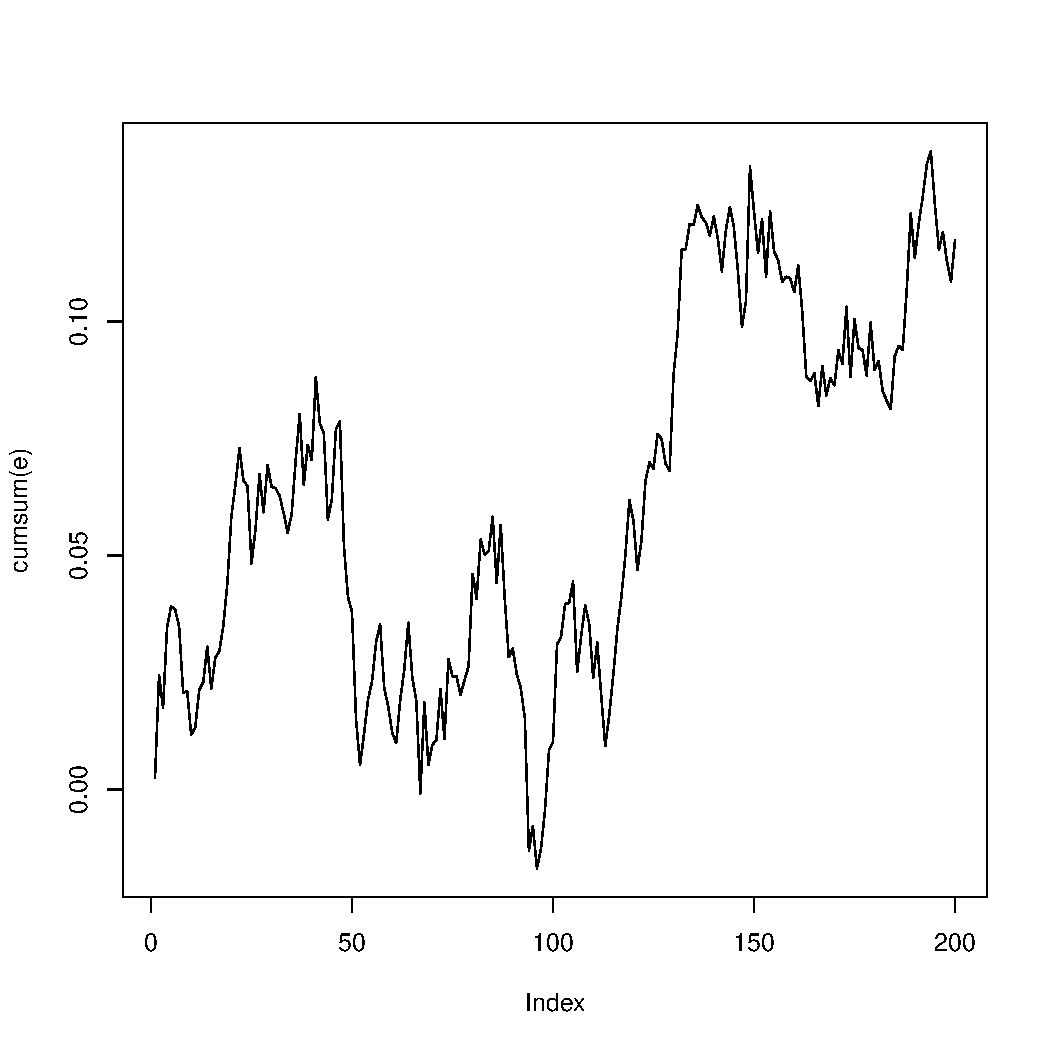
\includegraphics[scale=0.6]{P41.pdf}
    \caption*{根据200个间隔所产生的标准布朗运动的模拟路径}
    \label{fig:BrownMotion1}
\end{figure}

\qd{广义布朗运动(generalized Brownian motion),或算数布朗运动或广义维纳过程}:随机过程$x=(x_t)_{t \geqslant 0}$,其中$x_t=x_0+\mu t +\sigma z_t,t \geqslant 0$。参数$\mu$反映了过程在单位时间里的期望变化,叫做票一律或简单称为“漂移”(drift)。参数$\sigma^2$反映了过程未来的不确定性,被称为过程的方差率(variance rate)。参数$\sigma$被称为过程的波动率。

广义布朗运动继承了标准布朗运动的很多特征。例如,广义布朗运动同样是马尔科夫过程,广义布朗运动的路径是连续的但处处不可微。除非$\mu=0$,广义布朗运动不是一个鞅。广义布朗运动的路径可以通过选择时间点$0 \equiv t_0 <t_1 <t_2< \cdots <t_n$并迭代计算
$$x_{t_i}=x_{t_{i-1}}+\mu(t_i-t_{i-1})+\epsilon_i \sigma \sqrt{t_i-t_{i-1}},i=1,\cdots,n$$
而得到,在此$\epsilon_1,\cdots,\epsilon_n$从标准正态分布中独立抽取。

如果参数$\mu$和$\sigma$随时间以确定性的方式变动,那么这一过程被成为非时齐的广义布朗运动。这样的过程可以用微分的形式表示为
$$dx_t=\mu(t)dt+\sigma(t)dz_t$$
观察一个很短的间隔$[t,t+\Delta t]$,期望的变化近似于$\mu(t)\Delta t$,该变化的方差近似为$\sigma(t)^2 \Delta t$。更准确地讲,在任何间隔$[t,t']$的增量为
$$x_{t'}-x_t=\int_t^{t'}\mu(u)du+\int_t^{t'}\sigma(u)dz_u$$
最后一项积分就是所谓的随机积分,将在以后介绍。我们也将介绍一个定理,根据该定理,从时刻t起,积分$\int_t^{t'}\sigma(u)dz_u$是一个服从均值为0方差为$\int_t^{t'}\sigma(u)^2du$的随机变量。
\begin{figure}[H]
    \centering
    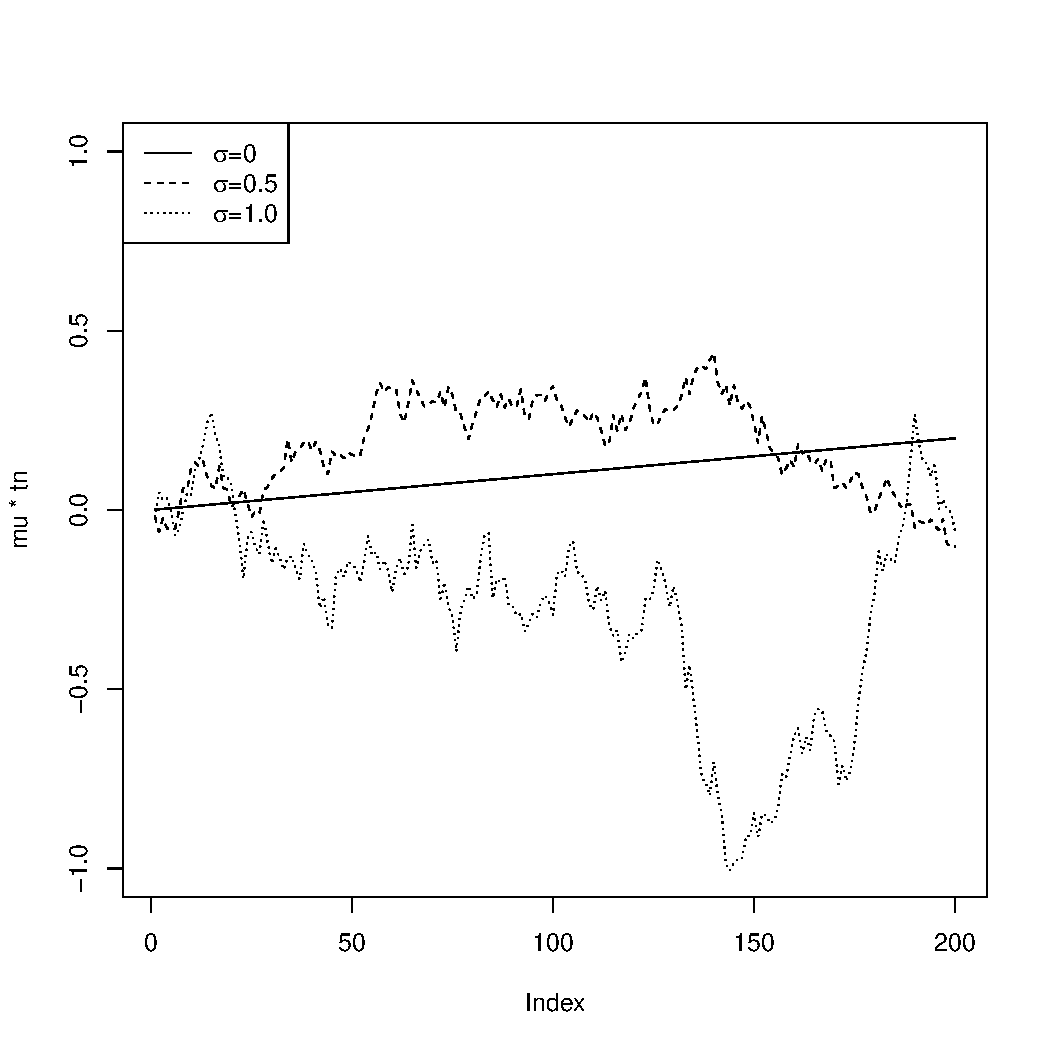
\includegraphics[scale=0.6]{P43.pdf}
    \caption*{广义布朗运动的模拟,其中$\mu=0.2,\sigma 1=0.5,\sigma 2=1.0$}
\end{figure}

\begin{lstlisting}[language=R]  
pdf(file="F:\\生活\\阅读材料\\固定收益建模\\FixedIncomeModelling.git\\trunk\\P43.pdf")
mu=0.2/200
sigma1=0.5
sigma2=1.0
r1 <- rnorm(200,mean=0,sd=sqrt(1/200))
r2 <- rnorm(200,mean=0,sd=sqrt(1/200))
tn <- 1:200
plot(mu*tn,type="l",ylim=c(-1,1))
lines(mu*tn+sigma1*cumsum(r1),type="l",lty=2)
lines(mu*tn+sigma2*cumsum(r2),type="l",lty=3)
legend("topleft",legend=expression(paste(sigma,"=0",sep=""),paste(sigma,"=0.5",sep=""),paste(sigma,"=1.0",sep="")),
       lty=c(1,2,3))
dev.off()
\end{lstlisting}

\subsection{扩散过程}

标准布朗运动和广义布朗运动的值空间等于$\mathbb{R}$。有些经济变量的取值只能是实数集$\mathbb{R}$的子集。例如,有限责任的金融资产价格不可能为负。我们使用扩散模型来呈现这样的变化。

一个随机过程$x=x(t)_{t \geqslant 0}$,对于无限短的时间间隔$[t,t+dt]$,其变化可以记为
$$dx_t=\mu(x_t,t)dt+\sigma(x_t,t)dz_t$$
该随机过程是一个(一维)的扩散过程,在此$z_t$是一个标准布朗运动,漂移$\mu$和波动率$\sigma$都是时间和随机过程当前值的函数。这一等式是对广义布朗运动微分方程的的扩展,广义布朗运动微分方程中,$\mu$和$\sigma$只是时间的函数,而扩散过程中两者是时间和随机过程当前值的函数。像这样等式两边都包含随机过程,叫做随机微分方程。因此,一个扩散过程就是一个随机微分方程的解。

如果$\mu$和$\sigma$都独立于时间,该扩散过程就是时齐的,反之则是非时齐的。对于一个时齐的扩散过程,未来值的分布将只取决于过程的当前值以及我们看到未来多远---而不是我们所处的时间点。

设想上式中,$dz_t$服从$N(0,dt)$分布,因此在无限短的时间间隔$[t,t+dt]$内,均值和方差分别为
$$E_t[dx_t]=\mu(x_t,t)dt,Var_t[dx_t]=\sigma(x_t,t)^2dt$$
其中$E_t[dx_t],Var_t[dx_t]$分别表示基于t时刻所能获得的信息的条件均值和方差。更准确地讲,扩散过程在仁和区间$[t,t']$内的变化为
$$x_{t'}-x_t=\int_t^{t'}\mu(x_u,u)du+\int_t^{t'}\sigma(x_u,u)dz_u$$
漂移和波动率实际上就是极限
$$\mu(x_t,t)=\lim\limits_{\Delta t \rightarrow 0} \frac{E_t[x_{t+\Delta t}-x_t]}{\Delta t}$$
$$\sigma(x_t,t)^2=\lim\limits_{\Delta t \rightarrow 0} \frac{Var_t[x_{t+\Delta t}-x_t]}{\Delta t}$$

一个扩散过程是一个马尔科夫过程。除非漂移$\mu(x_t,t)$对于所有的$x_t$和$t$都为0,否则扩散过程不是鞅。扩散过程的路径连续但处处不可微。扩散过程的值空间和未来值的分布将只依赖于函数$\mu$和$\sigma$。如果$\sigma(x,t)$连续且非0,那么由x生成的信息与z生成的信息是相同的,即$F^x=F^z$。
\end{document}


